\documentclass[12pt]{article}
\usepackage[margin=1in]{geometry}
\usepackage[all]{xy}

\usepackage{amsmath,amsthm,amssymb,color,latexsym, esint}
\usepackage{geometry}        
\geometry{letterpaper}    
\usepackage{graphicx}

\newcommand{\legendre}[2]{\ensuremath{\left( \frac{#1}{#2} \right) }}
\newtheorem{problem}{Problem}

\newenvironment{solution}[1][\it{Solution}]{\textbf{#1. } }{$\square$}


\begin{document}
\noindent Introduction to Fluid Dynamics \hfill Assignment 1\\
Yunzhe Zheng. (2025/09/13)

\hrulefill

\begin{problem}
    In 3D Cartesian coordinate $(x,y,z)$, show $(\textbf{u}\cdot\nabla)\textbf{u}=(\nabla\times\textbf{u})\times\textbf{u}+\nabla(\frac{1}{2}\textbf{u}\cdot\textbf{u})$.
\end{problem}

\textbf{Proof:} I shall prove it using Levi-Civita symbol, but first we should prove that 
$$
\epsilon_{ijk}\epsilon_{imn}=\delta_{jm}\delta_{kn}-\delta_{jn}\delta_{km}
$$
Observe that since $(\textbf{a}\times\textbf{b})\cdot(\textbf{c}\times\textbf{d})=(\textbf{a}\times\textbf{c})\cdot(\textbf{b}\times\textbf{d})$, where the LHS is $\sum\limits_{i}\epsilon_{ijk}\epsilon_{imn}a_jb_kc_md_n$. Also notice that in the RHS, terms are in the form of either $(a_mb_nc_md_n)$ or $(a_mb_nc_nd_m)$, then rewrite RHS by 
$$
    \sum\limits a_jc_m\delta_{jm}b_kd_n\delta_{kn}-\sum\limits a_jd_n\delta_{jn}b_kc_m\delta_{km} = \sum\limits a_jb_kc_md_n(\delta_{jm}\delta_{kn}-\delta_{jn}\delta_{km})
$$ thus we have the required equality. \\
\indent Now, we have 
\begin{align*}
    \left[(\nabla\times \textbf{u})\times \textbf{u}\right]_i&=\epsilon_{ijk}\left(\epsilon_{jmn}\frac{\partial u_n}{\partial x_m}\right)u_k =\epsilon_{jki}\epsilon_{jmn}\frac{\partial u_n}{\partial x_m}u_k \\
    &= (\delta_{km}\delta_{in}-\delta_{kn}\delta_{im})\frac{\partial u_n}{\partial x_m}u_k \\
    &=\delta_{km}\delta_{in}\frac{\partial u_n}{\partial x_m}u_k-\delta_{kn}\delta_{im}\frac{\partial u_n}{\partial x_m}u_k \\
    &= u_k\frac{\partial u_i}{x_k}-\frac{\partial u_k}{\partial x_i}u_k \\
    &= (\textbf{u}\cdot \nabla)u_i - \frac{\partial}{\partial x_i}\left(\frac{1}{2}\textbf{u}\cdot\textbf{u}\right)
\end{align*}
\qed
\\
\begin{problem}
    Whether a fluid is incompressible or not, each element must conserve its mass as it moves. Consider the rate of mass flow through a fixed surface $S$ drawn in the fluid. Show that this conservation of mass implies 
    $$
        \frac{\partial \rho}{\partial t} + \nabla\cdot(\rho\textbf{u})=0
    $$ where $\rho(\textbf{x}, t)$ denotes that density of the fluid. Show too that this equation may be alternatively be written 
    $$
        \frac{D\rho}{Dt}+\rho\nabla\cdot\textbf{u}=0
    $$
\end{problem}

\textbf{Proof:} Inspired by lecture note, we have 
$$
    (\textbf{u}\cdot\textbf{n})\Delta S = \frac{\Delta V}{\Delta t}
$$ multiply both sides by $\rho(\textbf{x}, t)$, then 
$$
    \rho(\textbf{u}\cdot\textbf{n})\Delta S=\frac{\Delta m}{\Delta t}
$$ By conservation of mass, we should have 
\begin{align*}
    -\frac{d}{dt}\iiint_{\Omega}\rho dV = \oiint_{\partial\Omega}(\textbf{u}\cdot\textbf{n})\rho ds \implies-\iiint_{\Omega}\frac{d\rho}{dt}dV=\iiint_{\Omega}\nabla\cdot(\rho\textbf{u})dV
\end{align*} by divergence formula, then move LHS to RHS and we obtain 
$$
    \frac{d\rho}{dt}+\nabla\cdot(\rho\textbf{u})=0
$$
\indent Moreover, since $\nabla\cdot (\rho\textbf{u})=\textbf{u}\cdot\nabla\rho+\rho(\nabla\cdot\textbf{u})$, plug in back to previous equation, we have 
$$
    \frac{d\rho}{dt}+\textbf{u}\cdot\nabla\rho+\rho(\nabla\cdot\textbf{u})=0 \implies \frac{D\rho}{dt}+\rho(\nabla\cdot\textbf{u})=0
$$ \qed
\\
\begin{problem}
    An ideal fluid is rotating under gravity $\textbf{g}$ with constant angular velocity $\Omega$, so that relative to fixed Cartesian axes $\textbf{u}=(-\Omega y,\Omega x, 0)$. We wish to find the surface of constant pressure. By Bernoulli, $\frac{p}{\rho}+\frac{1}{2}\textbf{u}\cdot\textbf{u}+gz$, so the constant pressure surfaces are 
    $$
        z= C-\frac{\Omega^2}{2g}(x^2+y^2)
    $$ for some constant $C$. What's wrong? Obtain the correct shape for the free surface.
\end{problem}

\textbf{Solution:} Since the given fluid is rotating, we can't use Bernoulli law for irrotational, steady, ideal flow and claim that Bernoulli quantity is conserved everywhere, we do can say that it is conserved along each streamline, but there is no way we can compare values on different streamlines. \\
\indent Plug $(-\Omega y, \Omega x, 0)$ into the component-wise Euler equation, we obtain 
$$
    \left\{\begin{matrix}
  -\Omega^2x=-\frac{1}{\rho}\frac{\partial P}{\partial x} \\
  -\Omega^2y=-\frac{1}{\rho}\frac{\partial P}{\partial y} \\
  -g = \frac{1}{\rho}\frac{\partial P}{\partial z}
\end{matrix}\right.
$$ then $P=\frac{1}{2}\rho\Omega^2(x^2+y^2)-\rho g z+C$, for some constant $C$, then the free surface will be 
$$
    z = \text{const} + \frac{1}{2g}\Omega^2(x^2+y^2).
$$ \qed
\\
\begin{problem}
    Take the Euler equation for an incompressible fluid of constant density, cast it into an appropriate form, and form suitable operation on it to obtain the energy equation:
    $$
        \frac{d}{dt}\int_{V}\frac{1}{2}\rho\textbf{u}^2dV=-\int_S\left(p'+\frac{1}{2}\rho\textbf{u}^2\right)\textbf{u}\cdot\textbf{n}dS
    $$ where $V$ is the region enclosed by a fixed closed surface $S$ drawn in the fluid, and $p'$ denotes $p+\rho\chi$, the non-hydrostatic part of the pressure field.
\end{problem}

\textbf{Solution:} We analyze the energy equation, where the LHS is simply
$$
    \int_{V}\frac{d}{dt}\frac{1}{2}\rho\textbf{u}^2dV=\int_{V}\rho\textbf{u}\cdot\frac{\partial}{\partial t}\textbf{u}dV
$$
Applying Divergence Theorem on the RHS gives us
\begin{align}
    -\int_V\nabla\cdot\left((p'+\frac{1}{2}\rho\textbf{u}^2)\textbf{u}\right)dV
\end{align}
Calculate the integrand of (1):
\begin{align*}
    \nabla\cdot\left((p'+\frac{1}{2}\rho\textbf{u}^2)\textbf{u}\right)&=\textbf{u}\cdot\nabla(p'+\frac{1}{2}\rho\textbf{u}^2)+(p'+\frac{1}{2}\rho\textbf{u}^2)(\nabla\cdot\textbf{u}) \\
    &=\textbf{u}\cdot \nabla p'+\frac{1}{2}\rho\textbf{u}\cdot\nabla\textbf{u}^2+0 \\
    &=\textbf{u}\cdot\nabla p-\textbf{u}\cdot\textbf{g}+\rho\textbf{u}\cdot(\textbf{u}\cdot\nabla)\textbf{u}
\end{align*} then 
\begin{align*}
    \rho\textbf{u}\cdot\frac{\partial\textbf{u}}{\partial t}=-\textbf{u}\cdot\nabla p + \textbf{u}\cdot\textbf{g} - \rho\textbf{u}\cdot(\textbf{u}\cdot\nabla)\textbf{u}
\end{align*} and we notice that we only need to modify Euler Equation by multiplying $\rho$ and dot product by $\textbf{u}$. \qed
\\
\begin{problem}
    Sketch the streamlines for the flow 
    $$
        u=\alpha x, v=-\alpha y, w=0
    $$
    where $\alpha$ is a positive constant. \\
    \indent Let the concentration of some pollutant in the fluid be 
    $$
        c(x,y,t)=\beta x^2ye^{-\alpha t}
    $$ for $y>0$, where $\beta$ is a constant. Does the pollutant concentration for any particular fluid element change with time? \\
    \indent An alternative way of describing any flow is to specify the position $x$ of each fluid element at time $t$ in terms of the position $\textbf{X}$ of that element at time $t=0$. For the above flow this 'Lagrangian' description is 
    $$
        x=Xe^\alpha t, y=Ye^{-\alpha t}, z=Z
    $$
    Verify by direct calculation that 
    $$
        \left(\frac{\partial \textbf{x}}{\partial t}\right)_{\textbf{X}}=\textbf{u}, \left(\frac{\partial\textbf{u}}{\partial t}\right)_{\textbf{X}}=\frac{D\textbf{u}}{Dt}
    $$ in this particular case. Why are these results true in general?
\end{problem}

\textbf{Solution:} By definition of streamline, we have 
$$
    \frac{dx}{u}=\frac{dy}{v} \implies \int\frac{dx}{\alpha x}=\int\frac{dy}{-\alpha y}
$$ then we have 
$$
    |y|=e^{-\ln{|x|}+\alpha C}=e^{\alpha C}\frac{1}{|x|}
$$ the sketch of streamlines would be: \\
\begin{center}
    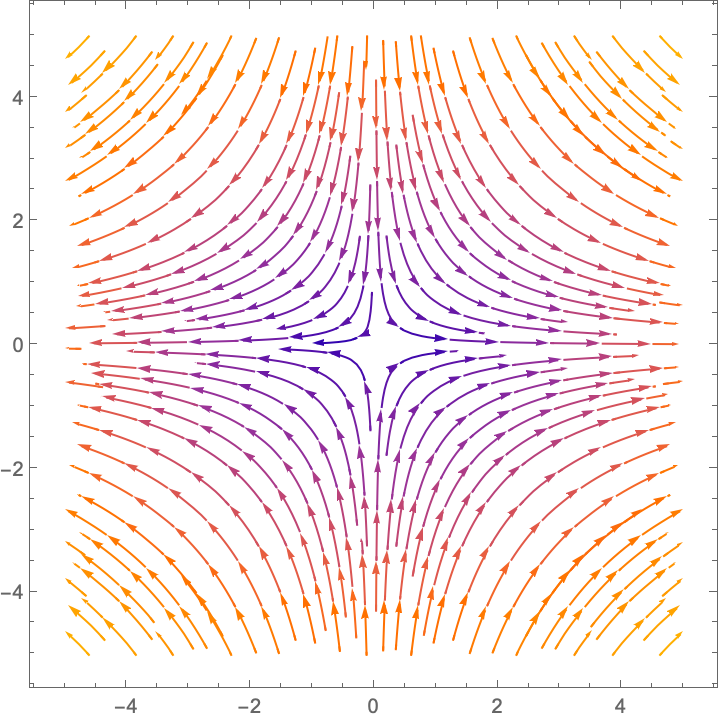
\includegraphics[scale=0.7]{images/streamline1.png}
\end{center}
\indent\indent To see the rate of change of the pollutant concentration, we calculate the material derivative of $c$
$$
    \frac{Dc}{Dt}=\frac{\partial c}{\partial t}+\textbf{u}\cdot\nabla c=-\alpha\beta x^2ye^{-at}+2\alpha\beta x^2ye^{-\alpha t}-\alpha\beta x^2ye^{-\alpha t} = 0
$$ then the concentration doesn't change with time. \\
\indent Finally, from direct calculation, we have
\begin{align*}
    \left(\frac{\partial x}{\partial t}\right)_{\textbf{X}}&=\alpha Xe^{\alpha t}=\alpha x \\
    \left(\frac{\partial y}{\partial t}\right)_{\textbf{X}}&=-\alpha Ye^{-\alpha t} = -\alpha y \\
    \left(\frac{\partial u}{\partial t}\right)_{\textbf{X}}&= \frac{\partial u}{\partial x}\frac{\partial x}{\partial t}=\alpha^2 x \\
    \left(\frac{\partial v}{\partial t}\right)_{\textbf{X}}&=\frac{\partial v}{\partial y}\frac{\partial y}{\partial t}=\alpha^2 y \\
    \frac{Du}{Dt}&=\frac{\partial u}{\partial t}+u\frac{\partial x}{\partial t} + v\frac{\partial y}{\partial t} + w\frac{\partial z}{\partial t}=\alpha^2 x \\
    \frac{Du}{Dt}&=\alpha^2 y
\end{align*} Thus the conclusion follows immediately. The result is true in general because the specified initial position $\textbf{X}$ is independent of $t$, such that we may substitute $\textbf{u}$ back after performing derivatives. \qed 
\\
\begin{problem}
    Consider the unsteady flow
    $$
        u=u_0, v=kt, w=0
    $$
    where $u_0$ and $k$ are positive constants. Show that the streamlines are straight lines, and sketch them at two different times. Also show that any fluid particle follows a parabolic path as time proceeds.
\end{problem}

\textbf{Proof:} By definition of streamline
$$
    \frac{dx}{u}=\frac{dy}{v}\implies \int\frac{dx}{u_0}=\int\frac{dy}{kt}
$$ then 
$$
    \frac{x}{u_0}=\frac{y}{kt}+C\implies y=\frac{k}{u_0}tx+\text{const} 
$$ are obviously straightlines. \\
\\
\indent Below are two sketches of two streamlines for two different $k$. \\
\begin{minipage}{0.45\textwidth}
  \centering
  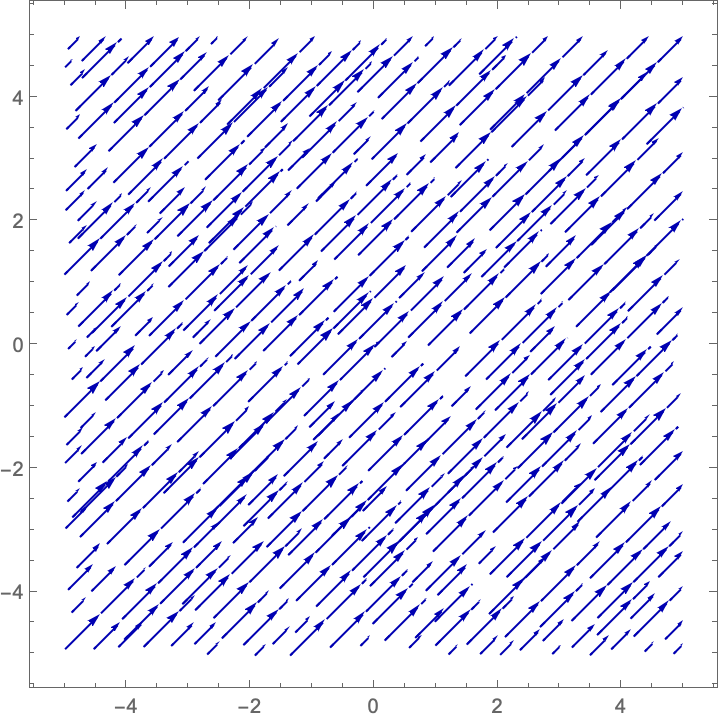
\includegraphics[scale=0.5]{images/streamline2.png}
\end{minipage}
\hfill
\begin{minipage}{0.45\textwidth}
  \centering
  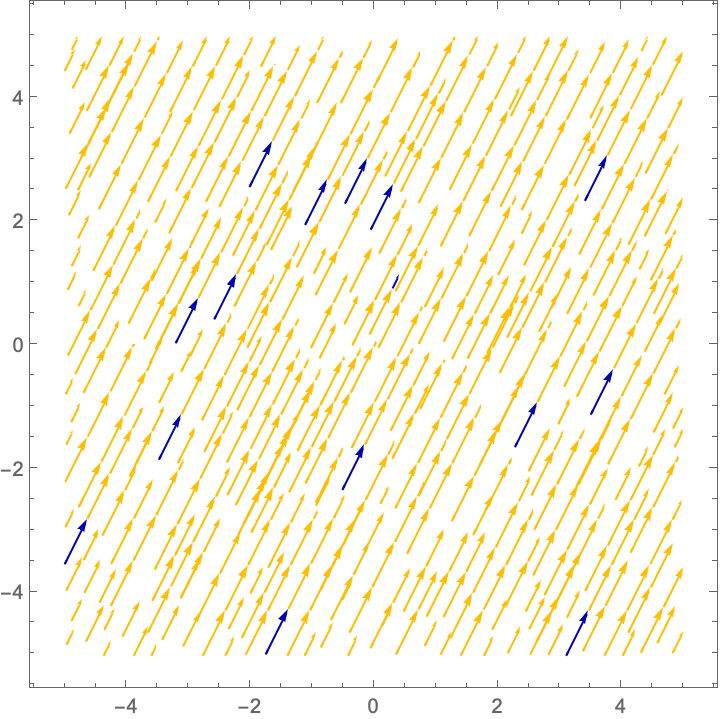
\includegraphics[scale=0.5]{images/streamline3.png}
\end{minipage}
\\
\indent Finally, we know that 
$$
    \left\{\begin{matrix}
  \frac{dx}{dt}=u_0 \\
  \frac{dy}{dt}=kt
    \end{matrix}\right. \implies
    \left\{\begin{matrix}
  x=u_0t + x_0\\
  y=\frac{1}{2}kt^2 + y_0
    \end{matrix}\right.
$$ where $(x_0, y_0)$ is the initial position of a particle, then 
$$
    y=\frac{1}{2}k\left(\frac{x-x_0}{u_0}\right)^2+y_0
$$ thus the trajectory is of the form of parabolic curve. \\
\qed
 
\end{document}